\documentclass{beamer}
\usepackage[utf8]{inputenc}
\usepackage[numbers]{natbib}
\usepackage{amsmath}
\usepackage{graphicx}
\usepackage{wrapfig}
\usepackage{lipsum}
\usepackage{siunitx}
\graphicspath{ {photo/} }

\usetheme{AnnArbor}
\usecolortheme{beaver}

%! Author = cyberstar
%! Date = 26.10.20
\title[Homemade Eye Tracker] %optional
{Constructing a Homemade Eye Tracker from Consumer-Grade Web Cameras}

\author[Sam, Kate] % (optional, for multiple authors)
{Samantha Aziz\inst{1} \and Kateryna Melnyk\inst{1}}

\institute[TXSU] % (optional)
{
\inst{1}%
Faculty of Computer Science\\
Texas State University
}

\date[10/28/20] % (optional)
{CS 7321 — Human Computer Interaction}

\begin{document}

    \frame{\titlepage}

    \begin{frame}
        \frametitle{Hardware: LifeCam VX-1000}

        \center
        For our experiment we use two cameras.
        Firstly, we modified a \textbf{Microsoft LifeCam VX-1000} to enable eye
        tracking functionality.

        \begin{figure}
            \begin{center}
                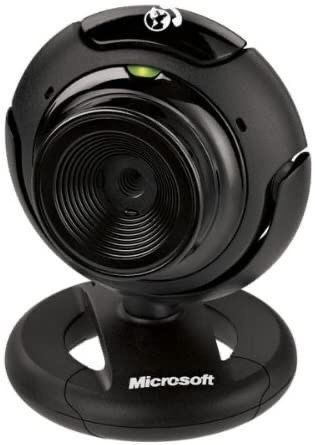
\includegraphics[width=0.2\textwidth]{VX_1000.jpg}
            \end{center}
            \caption{LifeCam VX-1000}
            \label{fig:VX_100.}
        \end{figure}

    \end{frame}

    \begin{frame}
        \frametitle{Hardware: ToLuLu 1080p webcam}
        \center Secondly, we continue our work with a \textbf{ToLuLu 1080p
        webcam.}

        \begin{figure}
            \begin{center}
                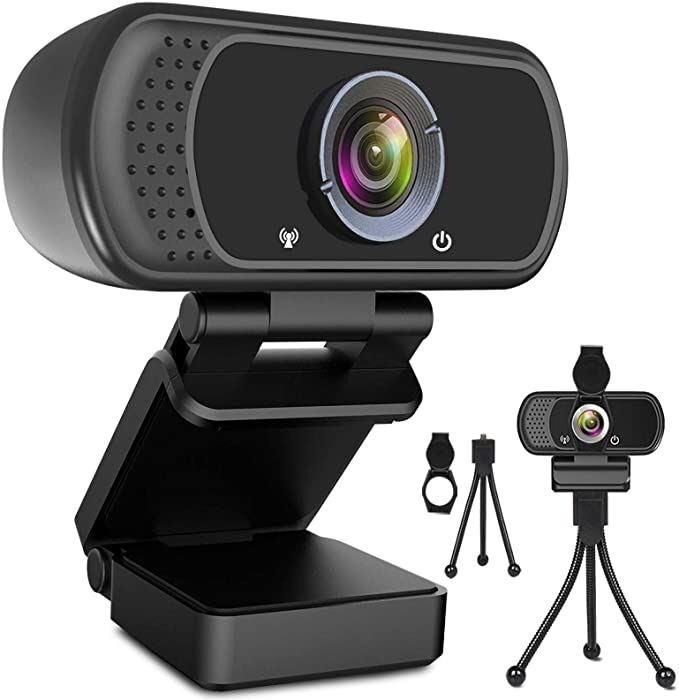
\includegraphics[width=0.4\textwidth]{ToLuLu.jpg}
            \end{center}
            \caption{ToLuLu 1080p webcam.}
            \label{fig:Tolulu}
        \end{figure}

    \end{frame}

    \begin{frame}
        \frametitle{Modification of the camera to remove IR filter}
        \center First, we removed the \textbf{IR} filter from the disassembled camera.

        \begin{figure}
            \begin{center}
                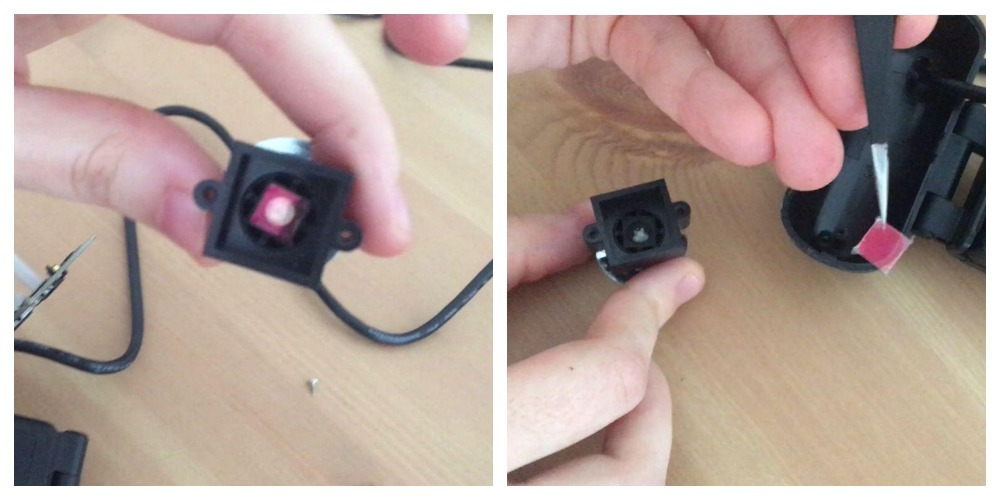
\includegraphics[width=0.8\textwidth]{Red_filter.jpg}
            \end{center}
            \caption{Camera with red filter and without it.}
            \label{fig:red_filter}
        \end{figure}

    \end{frame}

    \begin{frame}
        \frametitle{Insertion of the visible light filter}
        \center
        The visible light filter - \textbf{"Kodak GC Ultramax 400 ASA 24 Exposure
        35mm Color Film"}.

        \begin{figure}
            \begin{center}
                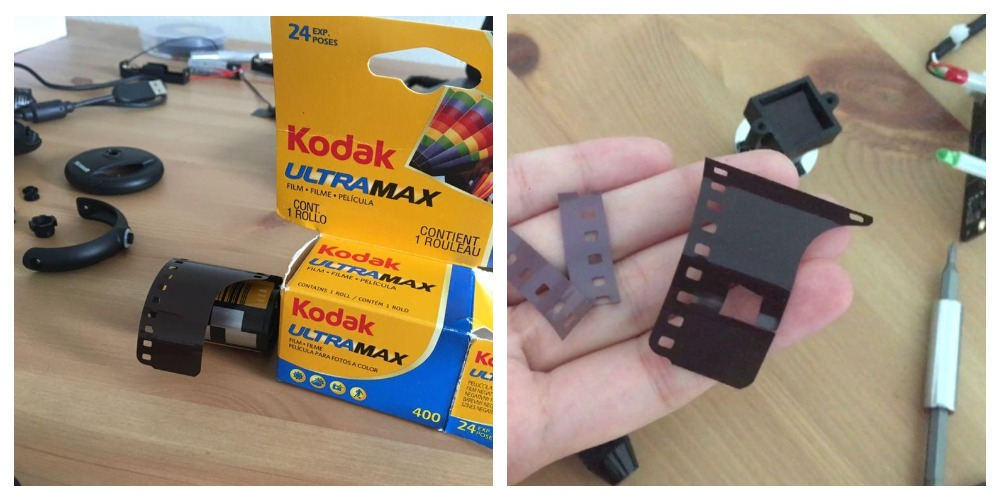
\includegraphics[width=0.8\textwidth]{Visible_light.jpg}
            \end{center}
            \caption{Visible light filter.}
            \label{fig:VL_filter}
        \end{figure}

    \end{frame}

    \begin{frame}
        \frametitle{Insertion of the visible light filter}
        \center

        We then replaced the \textbf{IR}(infra-red) filter with a sheet of
        exposed, undeveloped camera film to filter natural light.

        \begin{figure}
            \begin{center}
                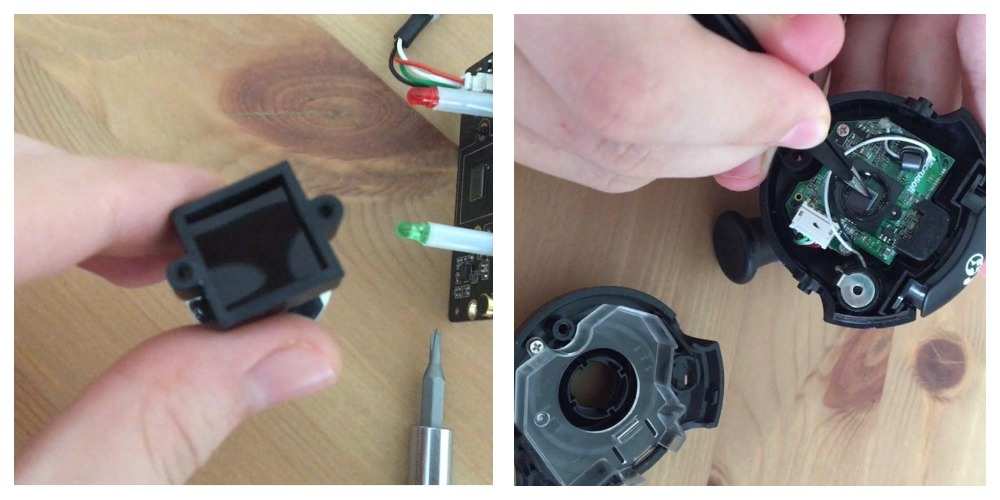
\includegraphics[width=0.8\textwidth]{VL_cameras.jpg}
            \end{center}
            \caption{Visible light filter in ToLuLu 1080p webcam and LifeCam
            VX-1000.}
            \label{fig:VL_cameras}
        \end{figure}

    \end{frame}

    \begin{frame}
        \frametitle{Assembly of the IR light}
        \center
        To improve tracking accuracy, we also attached a \textbf{1.5V infrared
        LED} to the top of the camera.

        \begin{figure}
            \begin{center}
                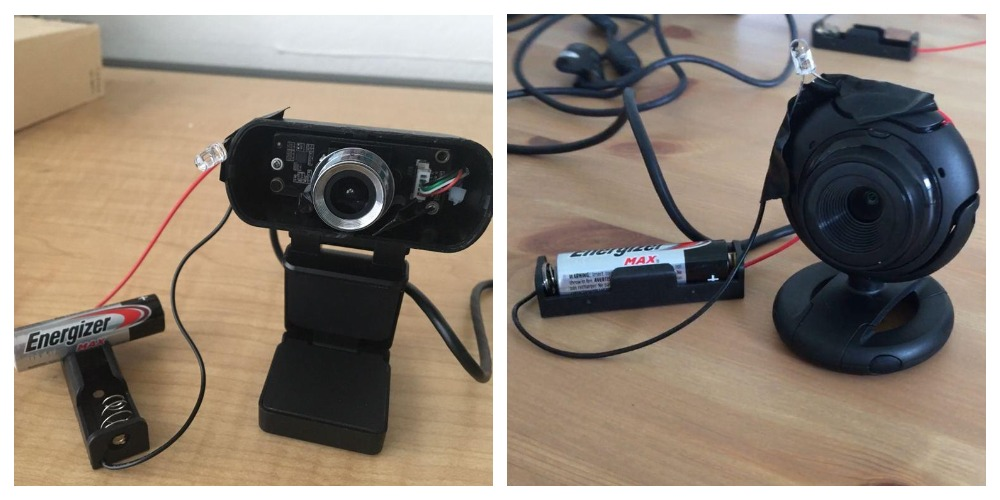
\includegraphics[width=0.8\textwidth]{IR_cameras.jpg}
            \end{center}
            \caption{The visible light filter in ToLuLu 1080p webcam
            and LifeCam VX-1000.}
            \label{fig:IR_cameras}
        \end{figure}

    \end{frame}

    \begin{frame}
        \frametitle{Software}

        \begin{itemize}
            \item Eye tracking and calibration was provided by the
            \textbf{ITU\_Gaze\_Tracker} codebase provided in class.
            \item This codebase was compiled in \textbf{Microsoft Visual Studio
            2017}.
            \item IT was executed on a \textbf{Dell Inspiron 7386} running
            \textbf{Windows 10}.
        \end{itemize}

    \end{frame}

    \begin{frame}
        \frametitle{Creation of camera holder, shin rest, and assembly of the
        IR light for ToLuLu 1080p webcam}

        \begin{figure}
            \begin{center}
                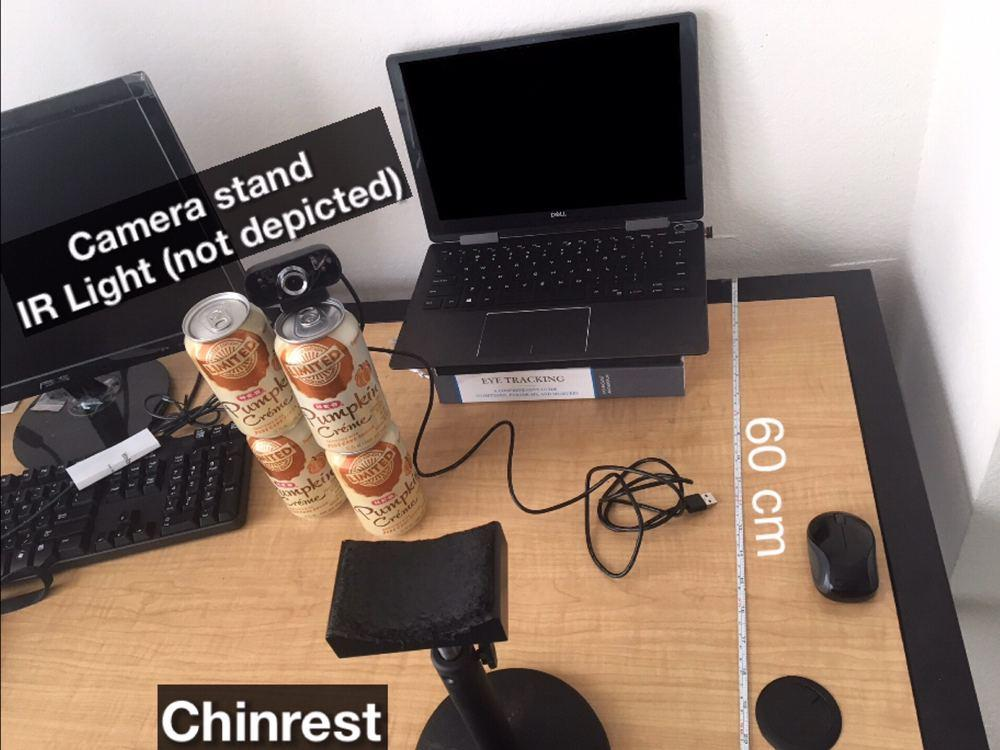
\includegraphics[width=0.7\textwidth]{Work_space_Tolulu.jpg}
            \end{center}
            \caption{The workspace with ToLuLu 1080p webcam}
            \label{fig:Workspace_Tolulu}
        \end{figure}

    \end{frame}

    \begin{frame}
        \frametitle{Creation of camera holder, shin rest, and assembly of the
        IR light for LifeCam VX-1000}

        \begin{figure}
            \begin{center}
                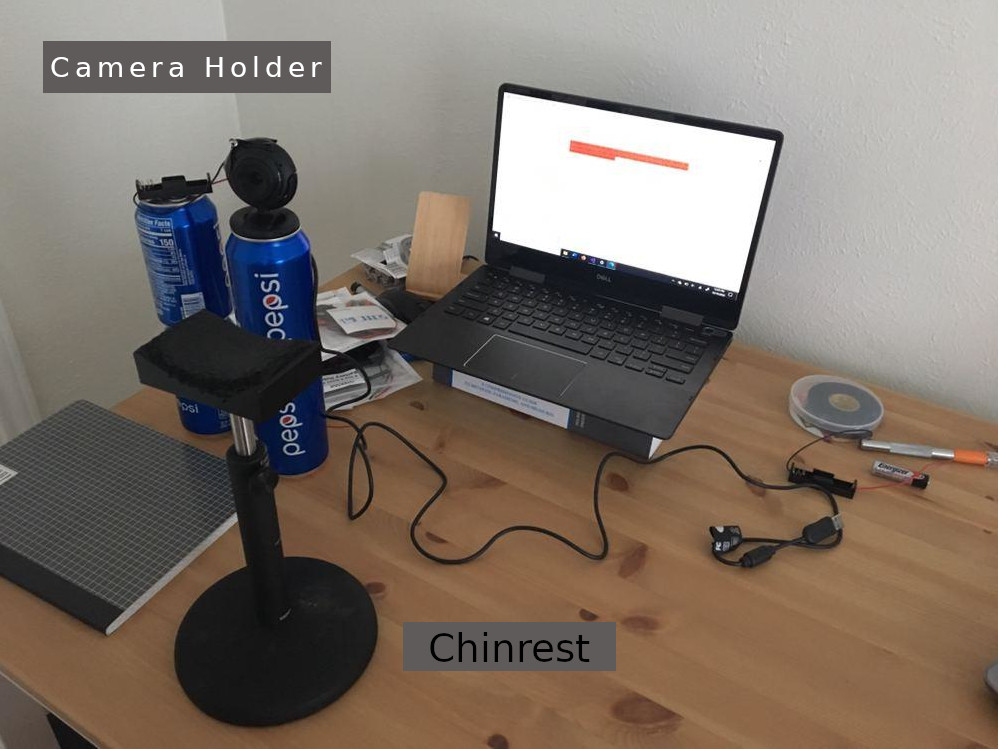
\includegraphics[width=0.7\textwidth]{Work_space_VX_1000.jpg}
            \end{center}
            \caption{The workspace with LifeCam VX-1000}
            \label{fig:Workspace_VX}
        \end{figure}

    \end{frame}

    \begin{frame}
        \frametitle{The best result that we were able to get with LifeCam VX-1000}

        \center
        The best \textbf{spatial accuracy}: \ang{1.6} \\
        The best \textbf{spatial precision}: \ang{1.2}

        \begin{figure}
            \begin{center}
                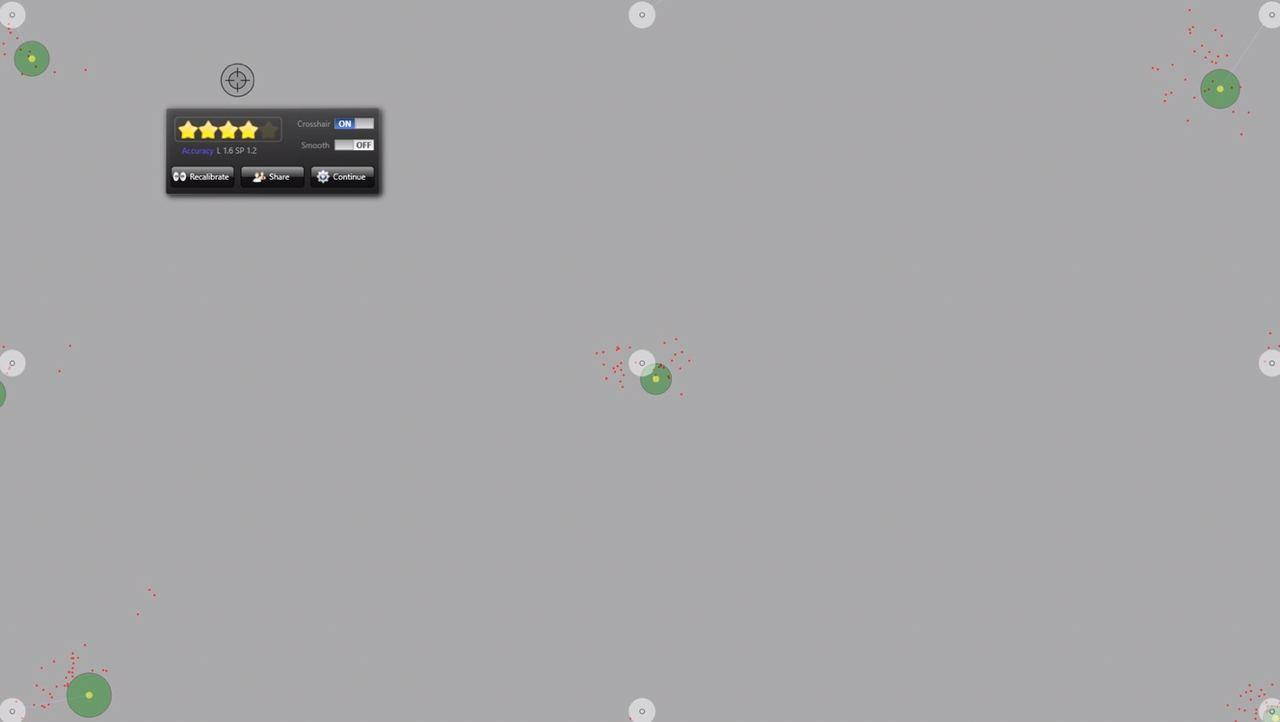
\includegraphics[width=0.7\textwidth]{Best_res_VX_1000.jpg}
            \end{center}
            \caption{The best results in experiment with LifeCam VX-1000.}
            \label{fig:Best_VX}
        \end{figure}

    \end{frame}

    \begin{frame}
        \frametitle{The best result that we were able to get with ToLuLu 1080p
        webcam}

        \center
        The best \textbf{spatial accuracy}: \ang{1.9} \\
        The best \textbf{spatial precision}: \ang{1.6}

        \begin{figure}
            \begin{center}
                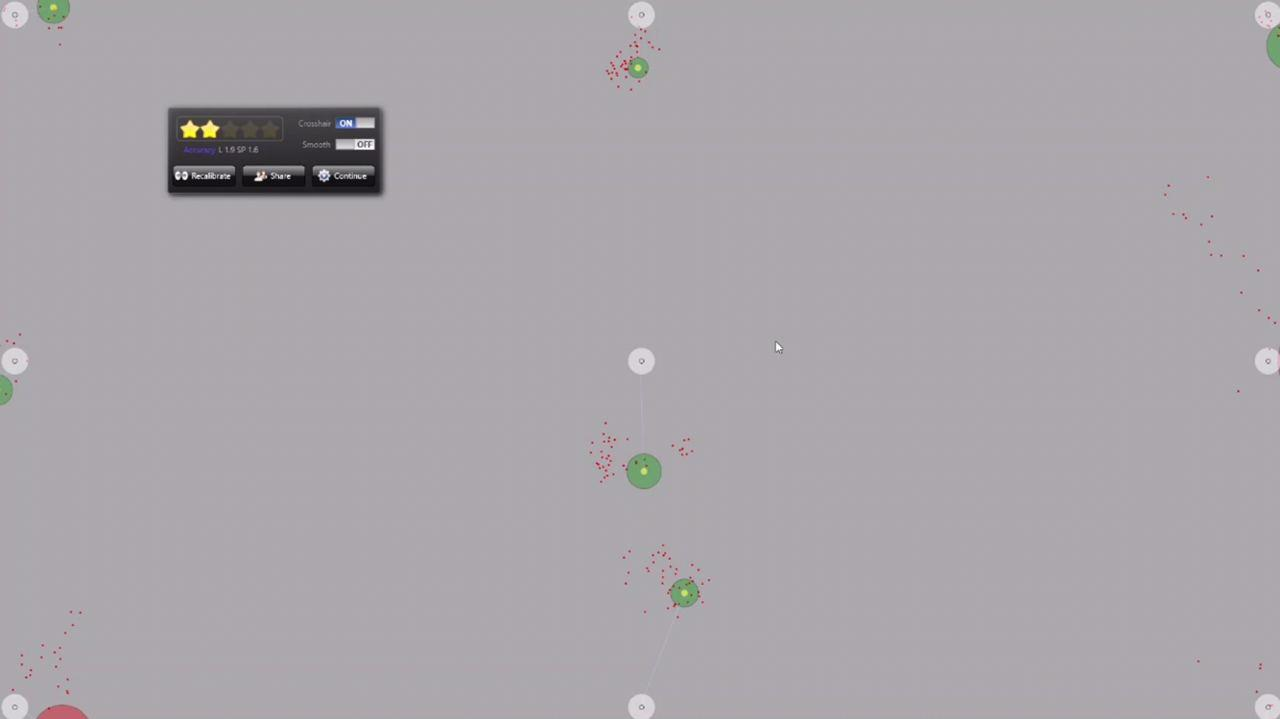
\includegraphics[width=0.7\textwidth]{Best_res_Tolulu.jpg}
            \end{center}
            \caption{The best results in experiment with ToLuLu 1080p webcam.}
            \label{fig:Best_Tolulu}
        \end{figure}

    \end{frame}

\end{document}